\documentclass[3p,times]{elsarticle}
%\usepackage{ecrc}
\usepackage{graphicx}
% used for flow charts
\usepackage{listings}
\usepackage{pgf}
\usepackage{tikz}
\usepackage{reotex}
\usepackage{algorithm}
\usepackage{algorithmic}
\usepackage{amssymb}
\usepackage{amsmath}
\usepackage{amsthm}

\usepackage[normalem]{ulem}
\usepackage{todonotes}
\usepackage{color}
\usepackage{verbatim}
\newcommand{\redt}[1]{\textcolor{red}{#1}}
\newcommand{\liyi}[1]{\textcolor{blue}{#1}}
%\newcommand{\xyz}[1]{\textcolor{blue}{#1}}

\newtheorem{example}{Example}[section]
\newtheorem{theorem}{Theorem}[section]
\newtheorem{lemma}{Lemma}[section]

\usepackage{url}
%\pagestyle{plain}
\begin{document}
\begin{frontmatter}
%\pagestyle{plain}
%\mainmatter

\title{Reasoning about Connectors in Coq}

%\titlerunning{Reasoning about Connectors in Coq}

\author{Xiyue Zhang, Weijiang Hong, Yi Li and Meng Sun}

%\authorrunning{X.~Zhang, W.~Hong, Y.~Li and M.~Sun}

\address{Department of Informatics and LMAM, School of Mathematical Sciences,\\ Peking University}
%\email{\{zhangxiyue,wj.hong,liyi\_math,sunm\}@pku.edu.cn}}

%\maketitle
\begin{abstract}
Reo is a channel-based exogenous coordination model in which complex coordinators, called connectors, are compositionally
built out of simpler ones. In this paper, we present a new approach to model connectors in Coq which is a proof assistant based on higher-order logic and $\lambda$-calculus.
The model reflects the original structure of connectors simply and clearly. In our framework, basic connectors (channels) are interpreted as axioms and composition operations are specified as inference rules. Furthermore, connectors are interpreted as logical predicates which describe the relation
between inputs and outputs. With such definitions provided, connector properties, as well as equivalence and refinement relations between different connectors, can be naturally formalized as \emph{goals} in Coq and easily proved using pre-defined \emph{tactics}. Particularly, to fulfil the proof of refinement relation, Z3, which can be used as a component in the context of other tools that require solving logical formulas, works as assistance.
%\paragraph*{Keywords:}

\end{abstract}
\begin{keyword}
Coordination language, Reo, Coq, Reasoning, Z3
\end{keyword}
\end{frontmatter}
\section{Introduction}\label{sec:introduction}

Modern software systems are typically distributed over large networks of computing devices, and usually the components
that comprise a system do not exactly fit together as pieces of a jigsaw puzzle, but leave significant interfacing gaps
that must somehow be filled with additional code. Compositional coordination models and languages provide a formalization
of the ``glue code" that interconnects the constituent components and organizes the mutual interactions among them in a
distributed processing environment, and played a crucial role for the success of component-based systems in the past decades.

As an example, Reo \cite{Arb04}, which is a channel-based model for exogenous coordination, offers
a powerful language for implementation of coordinating component connectors. Connectors provide the protocols that control and organize
the communication, synchronization and cooperation among the components that they interconnect. Primitive connectors, called {\em channels}
in Reo, can be composed to build complex connectors. Reo has been successfully applied in different application domains, such as
service-oriented computing and bioinformatics \cite{CCA04,SA07}. In recent years,
verifying the correctness of connectors is becoming a critical challenge, especially due to the advent of Cloud computing
technologies. The rapid growth of size and complexity of the computing infrastructures has made it more difficult to model
and verify connector properties, and thus leads to less confidence on the correctness of connectors.


Several works have been done for formal modeling and verifying
connectors. An operational semantics for Reo using Constraint Automata
(CA) was provided by Baier et al. \cite{BSAR06}, and later the symbolic model checker Vereofy \cite{BBK+10} was developed,
which can be used to check CTL-like properties.
% However, modeling unbounded primitives or even bounded primitives with unbounded
% data domains is impossible with finite constraint automata. Bounded large data domains cause an
% explosion in the constraint automata model which becomes problematic.
% A model for Reo connectors based on the idea of coloring a connector with possible data flows to
% resolve synchronization and exclusion constraints was presented by Clarke et al. \cite{CCA07}. Unlike the operational semantics,
% data sensitive behavior, which is supported by Reo, are not captured by the coloring approach.
Besides, one attractive approach is to translate from Reo to other formal models such as Alloy
\cite{KSA+08}, mCRL2 \cite{KKV12}, UTP \cite{AAA+09,SAA+12}, etc.,
which makes it possible to take advantage of existing verification
tools. A comparison of existing semantic models for Reo can be found
in \cite{JA12}.

In this paper, we aim to provide an approach to formally modeling and reasoning about connectors using Coq.
The basic idea of our
approach is to model the behavior of a connector by representing it as a logical predicate which describes the relation among
the timed data streams on the input and output nodes, and to reason about connectors' properties, as
well as the equivalence and refinement relations
between connectors, by using proof principles and tactics in Coq.
Compared with existing approaches for verifying connectors' properties \cite{BBK+10,KB09,KKV12}, using Coq is especially helpful when
we take infinite behavior into consideration. The coinductive proof principle makes it possible to prove connectors' properties easily while it
is difficult (sometimes impossible) for other approaches (like model checking) because of the huge (or maybe infinite) number of states. The main drawback of failing to check the complementary refinement relation in Coq is made up by Z3.
While Coq provides a platform to prove properties with a series of tactics and strategies to be considered, Z3 can be used as a component in the context of other tools that require solving logical formulas which is in consistent with the definition of Reo connectors.

This is not a brand new idea, as we have already provided a solution for modeling Reo in Coq in\cite{LS15}, where connectors are represented in a constructive way, and
verification is essentially based on simulations. We do believe that the approach in this paper is reasonably different from
its predecessor where Coq seldom shows its real power. To be more specific, our new work has its certain
advantanges comparing with \cite{LS15} in the following
aspects:
\begin{itemize}
\item {\bf Modeling Method:} We use axioms to describe basic channels and their composition operations, which is more natural on a proof-assistant
platform than the simulation-based approach in \cite{LS15}.
\item {\bf Expression Power:} Any valid Coq expression can be used to depict properties, which is obviously more powerful than just using LTL formulas in
\cite{LS15}. Furthermore, support for continuous time behavior is also
possible in our approach in this paper.
\item {\bf Refinement and Equivalence Checking:} In our framework, equivalence and refinement relations can be proved among different connectors, while the previous one is not capable of either equivalence or refinement checking.
\end{itemize}


The paper is organized as follows: After this general introduction, we briefly summarize Reo and Coq
in Section \ref{sec:pre}. Section \ref{sec:basicdef} shows the notion of timed data streams and some
pre-defined auxiliary functions and predicates. Section \ref{sec:channelandoperator} presents the
formal modeling of basic channels and operators, as well as complex connectors. Section
\ref{sec:verification} shows how to reason about connector properties and equivalence (or
refinement) relations in our framework. Section \ref{sec:refinement} concentrates on the proof of refinement relation between two connectors.
In Section \ref{sec:conclusion}, we concludes with some further research directions. Full source codes can be found at \cite{reo2coqfile} for further reference.

\section{Preliminaries}\label{sec:pre}

In this section, we provide a brief introduction to the coordination language Reo and proof assistant tools Coq and Z3.

\subsection{The Coordination Model Reo}
Reo is a channel-based exogenous coordination model wherein complex coordinators, called connectors,
are compositionally built out of simpler ones \cite{Arb04}.
Further details about Reo and its semantics can be found in \cite{Arb04,AR03,BSAR06}.
The simplest connectors are channels with well-defined behavior such as synchronous channels, FIFO channels, etc.
Each channel in Reo has exactly two directed ends, with their own identities.
There are two types of channel ends: source ends and sink ends. A source channel end accepts
data into the channel. A sink channel end dispenses data out of the channel.
\begin{figure}
  \centering
  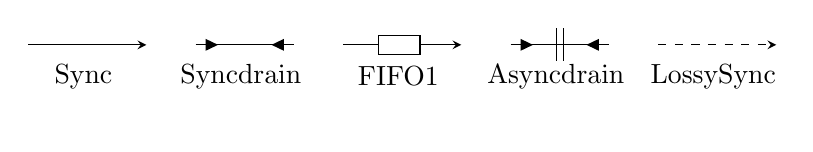
\begin{tikzpicture}
  \draw (0.7, 0.6) node[draw=none] {Sync};
  \sync{(0,1)}{(1.5,1)}{}
  \draw (2.7, 0.6) node[draw=none] {Syncdrain};
  \syncdrain{(2,1)}{(3.5,1)}{node[below]{}}
  \draw (4.7, 0.6) node[draw=none] {FIFO1};
  \fifoe{(4,1)}{(5.5,1)}{node[below]{}}
  \draw (6.7, 0.6) node[draw=none] {Asyncdrain};
  \asyncdrain{(6,1)}{(7.5,1)}{node[below left]{}}
  \draw (8.7, 0.6) node[draw=none] {LossySync};
  \lossysync{(8,1)}{(9.5,1)}{node[below left]{}}
  \end{tikzpicture}\vspace{-6mm}
  \caption{Five types of basic channels.}\label{fig:basicchannel}
\end{figure}


The graphical notations of some basic channels are presented in Fig. \ref{fig:basicchannel}, and their behavior can be interpreted as follows:
\begin{itemize}
\item{\textbf{Sync:} a synchronous channel with one source end and one sink end. The pair of I/O operations on its two ends can succeed only simultaneously.}
\item{\textbf{SyncDrain:} a synchronous channel which has two source ends.
 The pair of input operations on its two ends can succeed only simultaneously.
 All data items written to this channel are lost.}
\item{\textbf{FIFO$n$:} an asynchronous channel with one source end and one sink end, and a bounded buffer with capacity $n$.
It can accept data items from its source end. The accepted data items are kept in the internal buffer, and dispensed to
the sink end in FIFO order.
Especially, the FIFO$1$ channel is an instace of FIFO$n$ where the buffer capacity is 1.}
\item{\textbf{AsyncDrain:}  an asynchronous channel} which has two source ends. The channel guarantees that the operations on its two ends never succeed simultaneously. All data items written to this channel are lost.
\item{\textbf{LossySync:} a synchronous channel with one source end
    and one sink end. The source end always accepts all data items. If
    there is no matching output operation on the sink end of the
    channel at the time that a data item is accepted, then the data
    item is lost; otherwise, the channel transfers the data item
    exactly the same as a Sync channel, and the output operation at the sink end succeeds.}
\end{itemize}

\begin{figure}
\centering
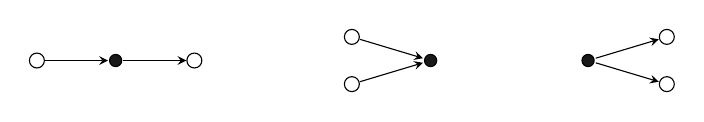
\begin{tikzpicture}
  \ionode{(io1)}{(0,5)}{}
  \ionode{(io2)}{(2,5)}{}
  \ionode{(io3)}{(4,4.7)}{}
  \ionode{(io4)}{(4,5.3)}{}
  \ionode{(io5)}{(8,4.7)}{}
  \ionode{(io6)}{(8,5.3)}{}
  \mixednode{(m1)}{(1,5)}{}
  \mixednode{(m2)}{(5,5)}{}
  \mixednode{(m3)}{(7,5)}{}
  \sync{(io1)}{(m1)}{}
  \sync{(m1)}{(io2)}{}
  \sync{(io3)}{(m2)}{}
  \sync{(io4)}{(m2)}{}
  \sync{(m3)}{(io5)}{}
  \sync{(m3)}{(io6)}{}
\end{tikzpicture}
\caption{Operations of channel composition.}\label{fig:channelcomposition}
\end{figure}

Complex connectors are constructed by composing simpler ones via the join and hiding operations. Channels are joined together in nodes. The set of channel ends coincident on a node is disjointly partitioned into the sets of source and sink channel ends that coincide on the node, respectively. Nodes are categorized into source, sink and mixed nodes, depending on whether all channel ends that coincide on a node are source ends, sink ends or a combination of the two. The hiding operation is used to hide the internal topology of a connector. The hidden nodes can no longer be accessed or observed from outside. There are three types of operations for channel composition: flow-through, merge and replicate. Fig. \ref{fig:channelcomposition} provides the graphical representation of these operations.

\subsection{The Proof Assistant tools}

Coq\cite{huet1997coq} is a widely-used proof assistant tool, where denotational formalizations (e.g.
theorem and hypothesis) and operational formalizations (e.g. functions and algorithms) are naturally
integrated. Moreover, it allows the interactive construction of formal proofs.
The formal language used in Coq is called \emph{Gallina}, which provides a convenient way to define
both programming statements and mathematical propositions, for example:
\begin{verbatim}
  (* a variable definition *)
  Variables a b: nat.
  (* a simple non-recursive function *)
  Definition inc(a:nat) := a + 1.
  (* axioms don't have to be proved *)
  Axiom inc_ax: forall c:nat, inc(c) > c.
  (* theorems rely on proving *)
  Theorem inc_eq: forall c:nat, inc(c) = c + 1.
  Proof.
    (* interactive proving based on tactics *)
    auto.
  Qed.
\end{verbatim}

As shown in this example, there are two rather different mode in Coq's interactive shell. When
we start Coq, we can write declarations and definitions in a functional-programming mode. Then, when
we start a \emph{Theorem}, or \emph{Lemma}, Coq jumps into the proving mode. We need to write
different \emph{tactics} to reduce the proving goal and finally finish the formal proof.

Furthermore, Coq is equipped with a set of well-written standard libraries. For example, as used in
this paper, \emph{List} describes the widely-used finite list structure, \emph{Stream} provides a co-inductive
definition of infinite lists, and \emph{Reals} defines various operations and theorems on real
numbers. Usually, quite a few lemmas and theorems are pre-defined in such libraries, making it
substantially easier to prove our goals.

%An abstract term has a type descriptor but no implementation, which is denoted as \emph{variables}
%or \emph{parameters}. Usually such terms are used to define theorems, e.g.
%\begin{verbatim}
  %Variables A B: Prop.
  %Theorem the: A -> B.
  %Proof.
    %...
  %Qed.
%\end{verbatim}
%In Contrast, an concrete term is more like a traditional function, e.g.
%\begin{verbatim}
  %Definition func(a:nat):nat := a + 1.
%\end{verbatim}
%An interesting feature of Coq is that both abstract and concrete terms can be unified in the same
%framework. For example, we can use \emph{Variable} to declare a function with no implementations.
%And such definitions are exactly equivalent with a proposition when both the arguments and the
%results are propositions. Similarly, a proof term, of a theorem of lemma, is a concrete term whose
%type is equal to the theorem.

%Besides, Coq provides a series of impressive libraries. For example, both \emph{Streams} and
%\emph{Reals} are already well-defined in Coq's standard library. Based on their work, we can prove
%many propositions more easily.


Z3\cite{MouraB08} is an efficient SMT Solver and a high performance theorem prover freely available from Microsoft Research. It can be used in various software verification and analysis applications. Acting as a SMT (Satisfiability Modulo Theories) solver, Z3 expands to deciding the satisfiability (or dually the validity) of first order formulas with respect to combinations of theories such as: arithmetic, bit-vectors, arrays, and uninterpreted functions. Given the data and time constraints of connectors, it allows us to decide the satisfiability against properties or refinement relations. Z3 provides bindings for several programming languages. In this paper, we use the Z3 API in Python to construct models and carry out experiments. The following example will provide an intuitive understanding of Z3 solver.
\begin{lstlisting}[frame=single]
x = Int('x')
y = Int('y')

s = Solver()
s.add(x > 10, Or(x + y > 3, x - y < 2))
#Solving constraints in the solver s
print s.check()

#Create a new scope
s.push()
s.add(y < 11)
#Solving updated set of constraints
print s.check()

#Restoring state
s.pop()
#Solving restored set of constraints
print s.check()
\end{lstlisting}
This example contains two constraints at first. From these two constraints, we can see that Z3 supports Boolean operators, such as \emph{And}, \emph{Or}, \emph{Not}, \emph{Implies (implication)}, apart from the operators like $<$, $>$ for comparison.
The command \emph{Solver()} creates a general purpose solver. Constraints can be added using the method \emph{add}. After being added to the solver, the constraints can be said having been asserted in the solver . The method \emph{check()} solves the asserted constraints. Finally, the result is satisfiable (unsatisfiable) if a solution was (not) found, respectively. A solver may fail to solve a system of constraints and \emph{unknown} is returned. Each solver maintains a stack of assertions. The command \emph{push} creates a new scope by saving the current stack size. The command \emph{pop} removes any assertion performed between it and the matching push.
\section{Basic Definitions}\label{sec:basicdef}

In this section, we briefly introduce the notion of timed data streams and some pre-defined auxiliary functions and predicates in Coq, which are used in the following sections for modeling connectors.

%\subsection{Timed data streams}
The behavior of a connector can be formalized by means of data-flows at its sink and source nodes which are essentially infinite sequences. With the help of the stream library in Coq, such infinite data-flows can be defined as \emph{timed data streams}:
\begin{verbatim}
    Definition Time := R.
    Definition Data := nat.
    (*Inductive Data : Set :=
        |Natdata : nat-> Data
        |Empty : Data.*)
    Definition TD := Time * Data.
    Variable Input : Stream TD.
    Variable Output : Stream TD.
\end{verbatim}
%
In our framework, time is represented by real numbers. Benefit from the completeness of real number system, we can express and carry out the effective operation of a quantity at any precision request.
The continuity of the set of real numbers is sufficiently enough for our modeling approach. Also the
continuous time model is more appropriate since it is very expressive and closer to the nature of time in the real world. Thus, the time sequence consists of increasing and diverging time moments. For simplicity, here we take the natural numbers as the definition of data, which can be easily expanded according to different application domains. The Cartesian product of time and data defines a TD object.
We use the stream module in Coq to produce streams of TD objects.

%\subsection{Auxiliary functions and predicates}
Some auxiliary functions and predicates are defined to facilitate the representation of axioms for basic channels in Reo. This part can be extended for further use in different problems.

The terms ``PrL" and ``PrR" take a pair of values (a, b) that has Cartesian product type A $\times$ B as the argument and return the first or second value of the pair, respectively.
%\begin{verbatim}
%    Definition PrL {A B: Type}(pair: A * B) := (...).
%    Definition PrR {A B: Type}(pair: A * B) := (...).
%\end{verbatim}

The following functions provide some judgment of time, which can make
the description of axioms and theorems for connectors more concise and
clear. ``Teq" means that time of two streams are equal and ``Tneq" has the
opposite meaning. ``Tle"  (``Tgt") represents that time of the first stream is
strictly less (greater) than the second stream. The judgement about
equality of data is analogous to the judgement of time. The complete
definition of these functions can be found at \cite{reo2coqfile}.


\section{Formal Modeling of Basic Channels and Operators}\label{sec:channelandoperator}
In this section, we show how primitive connectors, i.e., channels, and operators for connector composition are specified in Coq and used for modeling of complex connectors. Then we can apply the tactics provided in Coq to reason about connector properties. Basic channels, which can be regarded as axioms of the whole framework, are specified as logical predicates illustrating the relation between the timed data streams of input and output. When we need to construct a more complex connector, appropriate composition operators are applied depending on the topological structure of the connector.

\subsection{Formal Modeling of Basic Channels}

We use a pair of predicates to describe the constraints on time and data, respectively, and their intersection to provide the complete specification of basic channels. This model offers convenience for the analysis and proof of connector properties. In the following, we present a few examples of the formal model of basic channels.

The simplest form of a synchronous channel is denoted by the Sync channel type. For a channel of the Sync type, a read operation on
its sink end succeeds only if there is a write operation pending on its source end. Thus, the time and data of a stream flowing
into the channel are exactly the same as the stream that flows out of the channel
\footnote{If we use $\alpha,\beta$ to denote the data streams that flow through the channel ends of a channel and $a,b$ to denote the time stream corresponding to the data streams, i.e., the $i$-th element $a(i)$ in $a$ denotes exactly the time moment of the occurrence of $\alpha(i)$, then we can easily obtain the specifications for different channels, as discussed in \cite{Sun12,SAA+12}. For example, a synchronous channel can be expressed as $\alpha=\beta \wedge \emph{a}=\emph{b}$.}.
The Sync channel can be defined as follows in the Coq system:
\begin{verbatim}
    Definition Sync (Input Output:Stream TD) : Prop :=
    Teq Input Output /\ Deq Input Output.
\end{verbatim}


The channel of type SyncDrain is a synchronous channel that allows pairs of write operations pending on its two ends to succeed simultaneously. All written data items are lost. Thus, the SyncDrain channel is used for synchronising two timed data streams on its two source ends. This channel type is an important basic synchronization building block for the construction of more complex connectors. The SyncDrain channel can be defined as follows:
\begin{verbatim}
    Definition SyncDrain (Input Output:Stream TD) : Prop :=
    Teq Input Output.
\end{verbatim}


The channel types FIFO and FIFO$n$ where $n$ is an integer greater than $0$ represent the
typical unbounded and bounded asynchronous FIFO channels. A write to a FIFO channel always succeeds, and a write to a FIFO$n$ channel succeeds only if the
number of data items in its buffer is less than its bounded capacity $n$. A read or take from a FIFO or FIFO$n$ channel suspends until the first data item
in the channel buffer can be obtained and then the operation succeeds.
%We use the $\overrightarrow{\emph{a}}$ to denote the tail of  a sequence \emph{a}.
For simplicity, we take the FIFO1 channel as an example. This channel type requires that the time when it consumes a data item through its source end is earlier than the time when the data item is delivered through its sink end. Besides, as the buffer has the capacity 1, time of the next data item that flows in should be later than the time when the data in the buffer is delivered. We use intersection of predicates in its definition as follows:
\begin{verbatim}
    Definition FIFO1(Input Output:Stream TD) : Prop :=
    Tle Input Output /\ Tle Output (tl Input)
    /\ Deq Input Output.
\end{verbatim}

For a FIFO1 channel whose buffer already contains a data element \emph{e}, the communication can be initiated only if the data element \emph{e} can be taken via the sink end. In this case, the data stream that flows out of the channel should get an extra element \emph{e} settled at the beginning of the stream. And time of the stream that flows into the channel should be earlier than time of the tail of the stream that flows out. But as the buffer contains the data element \emph{e}, new data can be written into the channel only after the element \emph{e} has been taken. Therefore, time of the stream that flows out is earlier than time of the stream that flows in. The channel can be represented as the intersection of several predicates as follows:
\begin{verbatim}
    Definition FIFO1e(Input Output:Stream TD)(e:Data) : Prop :=
    Tgt Input Output /\ Tle Input (tl Output)
    /\ PrR (hd Output) = e  /\ Deq Input (tl Output).
\end{verbatim}

In the following we choose Axiom to define LossySync and AsyncDrain
because it is easier to use the coinductive expression to specify
their behavior.

A LossySync channel behaves the same as a Sync channel, except that a write operation on its source always succeeds immediately. If a compatible read or take operation is already pending on the sink of a LossySync channel, the written data item is transferred to the pending operation and both succeed. Otherwise, the write operation succeeds and the data item is lost. The LossySync channel can be defined as follows:
\begin{verbatim}
   Parameter LossySync: Stream TD -> Stream TD -> Prop.
   Axiom LossySync_coind:
     forall Input Output: Stream TD,
     LossySync Input Output ->
       (
        (hd Output = hd Input  /\ LossySync (tl Input)(tl Output))
        \/
        LossySync(tl Input) Output
       ).
\end{verbatim}

AsyncDrain is analogous to SyncDrain except that it guarantees that the pairs of write operations on the two channel ends never succeed simultaneously. Similarly it only has requirements on the time of the two streams on its opposite ends, but it requires that the times of the two streams are always different. The AsyncDrain channel can be defined as follows:
\begin{verbatim}
    Parameter AsyncDrain: Stream TD -> Stream TD -> Prop.
    Axiom AsyncDrain_coind:
      forall Input1 Input2: Stream TD,
      AsyncDrain Input1 Input2 ->
        (~ PrL(hd Input1)  =  PrL (hd Input2) )
        /\
        ( (
          (PrL(hd Input1) < PrL (hd Input2)) /\
          AsyncDrain (tl Input1) Input2
          ) /\
          (
          (PrL(hd Input1) > PrL (hd Input2))  /\
          AsyncDrain Input1 (tl Input2)
          )
        ).
\end{verbatim}

Defining basic channels by intersection of predicates provides the following benefits:
\begin{itemize}
\item Firstly, this makes the model intuitive and concise as each predicate describes a simple order relation on time or data.
\item Secondly, we can easily split predicates for proofs of different properties which can make the proving process simpler.
\end{itemize}
%Each predicate can be viewed as an atom. The theorems and propositions which will be described later are also illustrated by atomic expressions.

\subsection{Formal modeling of Operators}
We have just described the way to define channel types, by means of definitions in Coq. Now we start defining the composition operators for connector construction. There are three types of composition operators for connector construction, which are \emph{flow-through}, \emph{replicate} and \emph{merge}, respectively.

The flow-through operator simply allows data items to flow through the junction node, from one channel to the other. We need not to give the flow-through operator a specific definition in the Coq system. For example, while we illustrate two channels \emph{Sync(A,B)} and \emph{FIFO1(B,C)}, a flow-through operator that acts on node \emph{B} for these two channels has been achieved implicitly.

%The property of replicate operator in Reo can be seen in the composition of two channels \emph{ab},\emph{cd}.
The replicate operator puts the source ends of different channels together into one common node, and a write operation on this node succeeds only if all the channels are capable of consuming a copy of the written data. %And the two channel ends are interchangeable.
Similar to the flow-through operator, it can be implicitly represented by the structure of connectors. For example, for two channels \emph{Sync(A,B)} and \emph{FIFO1(C,D)}, we can illustrate \emph{Sync(A,B)} and \emph{FIFO1(A,D)} in Coq instead of defining a function like \emph{rep(Sync(A,B),FIFO1(C,D))} and the replicate operator is achieved directly by renaming \emph{C} with \emph{A} for the FIFO1 channel.

The merge operator is more complicated. We consider merging two
channels \emph{AB} and \emph{CD}. When the merge operator acts on
these two channels, it leads to a choice of taking from the common
node that delivers a data item out of \emph{AB} or \emph{CD}.
%If both channels have data items available, the choice is
%non-deterministic\footnote{Choices are made by external context, so
%the definition here remains deterministic.}.
Similar to the definition of basic channels, we define merge as the intersection of two predicates and use recursive definition here:
%    Definition xor(a b: Prop) :=  (a \/ b) /\ ~(a /\ b).
\begin{verbatim}
    Parameter merge:
    Stream TD -> Stream TD ->Stream TD -> Prop.
    Axiom merge_coind:
      forall s1 s2 s3:Stream TD,
      merge s1 s2 s3-> (
        ~ (PrL(hd s1) = PrL(hd s2)) /\
        (
          (PrL(hd s1) < PrL(hd s2)) ->
          ((hd s3 = hd s1)  /\ merge (tl s1) s2 (tl s3))
        ) /\ (
          (PrL(hd s1) > PrL(hd s2)) ->
          ((hd s3 = hd s2)  /\ merge s1 (tl s2) (tl s3))
        )
      ).
\end{verbatim}

\begin{figure}
\vspace{0cm}
\centering
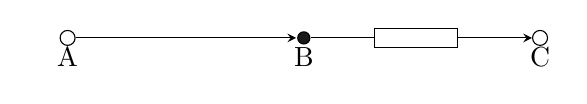
\begin{tikzpicture}
\ionode{(io1)}{(0.5,0)}{node[below]{A}}
\ionode{(io2)}{(6.5,0)}{node[below]{C}}
\mixednode{(m1)}{(3.5,0)}{node[below]{B}}
\sync{(io1)}{(m1)}{}
\fifoe{(m1)}{(io2)}{}
\end{tikzpicture}
\caption{A connector consisting of a Sync channel and a FIFO1 channel.}\label{fig:compsyncfifo}
\end{figure}

Based on the definition of basic channels and operators, more complex connectors can be constructed structurally.
%As the whole structure of each connector has been determined, the rest work is to use the operators to connect appropriate  channels according to the structure of each connector.
To show how a composite connector is constructed, we consider a simple example as shown in Fig. \ref{fig:compsyncfifo}, where a FIFO1 channel is attached
to the sink end of a Sync channel. Assume \emph{AB} is of type Sync and \emph{BC} is of type FIFO1, then we can construct the required connector by
illustrating \emph{Sync(A,B)} and \emph{FIFO1(B,C)}. The configuration and the functionality of the required connector can be specified using this concise method. Note that the composition operations can be easily generalized to the case of multiple nodes, where the modeling of connectors is similar. More
examples can be found in Section \ref{sec:verification}.






\section{Reasoning about Connectors}\label{sec:verification}
After modeling a connector in Coq, we can analyse and prove important properties of the connector. In this section, we give some examples to elucidate how to
reason about connector properties and prove refinement/equivalence relations between different connectors, with the help of Coq.


\subsection{Derivation of Connector Properties}
The proof process of a property is as follows: the user states the proposition that needs to be proved, called a \emph{goal},
then he/she applies commands called \emph{tactics} to decompose this goal into simpler subgoals or solve it directly. This decomposition
process ends when all subgoals are completely solved. In the following, we use some examples to illustrate our approach instead of
giving all the complex technical details.
\begin{example}
We first consider the connector given in Fig. \ref{fig:compsyncfifo}, which consists of two channels \emph{AB} and \emph{BC} with types Sync and FIFO1, respectively.

We use $a$ and $b$ to denote the time streams when the corresponding data streams flow into and out of the Sync channel \emph{AB}, and
\emph{c} to denote the time stream for the data stream that flows out of the FIFO1 channel \emph{BC}. Here we can see that a flow-through
operation has acted on the mixed node \emph{B}. The time when the stream flows into the FIFO1 channel \emph{BC} is equal to the time when the
stream flows out of the Sync channel \emph{AB}. The following theorem states the property $a < c$ for this connector. The connector is based on the
axioms Sync and FIFO1, which can be used as hypotheses for the proof of the theorem.
\begin{theorem}\label{the:tleac}
$\forall A,B,C.\:Sync(A,B)\land FIFO1(B,C) \rightarrow Tle(A,C)$.
\end{theorem}

In Coq, the theorem can be proved as follows:
\begin{verbatim}
    Theorem test1: forall A B C,
      Sync A B /\ FIFO1 B C -> Tle A C.
    Proof.
        intros. destruct H. destruct H0.
        intro n. rewrite H. apply H0.
    Qed.
\end{verbatim}

First we give the Coq system a proposition
\texttt{test1} which needs to be proved. The proposition is represented by a logical expression.
Table \ref{test1} shows the detailed proving steps and the feedback that the Coq system provides during the proof.
\begin{table}
\newcommand{\tabincell}[2]{\begin{tabular}{@{}#1@{}}#2\end{tabular}}
  \centering
  \caption{Steps and feedbacks for proving Theorem \ref{the:tleac}}
  \begin{tabular}{|c|c|c|}\hline
\tabincell{c}{Step} & \tabincell{c}{Feedback}\\\hline
\tabincell{c}{Theorem test1:\\\emph{forall A B C,} \\ \emph{Sync A B $\rightarrow$ FIFO1 B C}
   \\ \emph{$\rightarrow$  Tle A C.}} & \tabincell{c}{ 1 subgoal:\\ \emph{forall A B C,} \\ \emph{Sync A B $\rightarrow$ FIFO1 B C  $\rightarrow$ Tle A C} } \\\hline
\tabincell{c}{intros } & \tabincell{c}{ 1 subgoal: \emph{Tle A C} \\ \emph{H : Sync A B;
H0 : FIFO1 B C}} \\\hline
\tabincell{c}{destruct \emph{H} } & \tabincell{c}{ 1 subgoal:  \emph{Tle A C} \\ \emph{H : Teq A B;
H1 : Deq A B;}  \\ \emph{H0 : FIFO1 B C}} \\\hline
\tabincell{c}{destruct \emph{H0} } & \tabincell{c}{ 1 subgoal: \emph{Tle A C} \\ \emph{H : Teq A B;
H1 : Deq A B;}\\ \emph{
H0 : Tle B C; H2 : Tle C (tl B) $\wedge$ Deq B C }}\\ \hline
\tabincell{c}{intro \emph{n} } & \tabincell{c}{ 1 subgoal: \emph{PrL (Str\_nth n A) $<$ PrL (Str\_nth n C)} \\ \emph{H : Teq A B;
H1 : Deq A B;
H0 : Tle B C; }\\
\emph{H2 : Tle C (tl B)$\wedge$ Deq B C}} \\\hline
\tabincell{c}{rewrite \emph{H}} & \tabincell{c}{ 1 subgoal: \emph{PrL (Str\_nth n B) $<$ PrL (Str\_nth n C) }\\ \emph{H : Teq A B;
H0 : Deq A B;
H1 : Tle B C;}\\
\emph{H2 : Tle C (tl B)$\wedge$Deq B C;
n : nat}} \\\hline
\tabincell{c}{apply \emph{H0} } & \tabincell{c}{ No more subgoals} \\\hline
\end{tabular}
\label{test1}
\end{table}

The advantages of using intersection of logical predicates to describe basic channels have emerged while proving this example.
After constructing the new connector, we use ``intros'' to split conditions and conclusions. Then we can use ``destruct" to obtain the conditions for time and data separately,
and make the proving procedure much more convenient. Once the concrete conditions are obtained, using ``intro"
contributes to comparing each time point in a sequence element by element. Then by using ``rewrite" \emph{H}, we can make
the proof a step forward with known conditions of the comparison of time \emph{a} and \emph{b}, and finally by
``apply" \emph{H0} we can prove the goal. This is the implementation for reasoning about the constructed connector.
Note that proper selection of strategies and tactics is essential for the proof of connector properties.
\end{example}

\begin{example}\label{ex:alternator}
In this example, we show a more interesting connector named \emph{alternator} which consists of three channels \emph{AB}, \emph{AC} and \emph{BC} of type Syncdrain, FIFO1 and Sync, respectively. With the help of this connector, we can get data from node \emph{B} and \emph{A} alternatively at node \emph{C}.
By using the axioms for the basic channels and operators of composition, we can get the connector as shown in Figure \ref{fig:alternator}(b). The two
channels \emph{AC} and \emph{BC} are merged together at node \emph{C}. Before the merge operation, the connector's structure is as shown in
Figure \ref{fig:alternator}(a), which is useful in the reasoning about the alternator.

%Prior to prove the property of the alternator, we first show a transformed version of the property mentioned above. It will be useful in the proof of the property of alternator. The transformed version consists of three channels. \emph{AB}, \emph{AC1} and \emph{BC2} are of type Syncdrain, FIFO1 and Sync which are shown on the left side of Figure \ref{alternator}.

We first introduce some lemmas to facilitate the proof.
\begin{verbatim}
    Lemma transfer_eq : forall s1 s2 s3 : Stream TD,
    ((Teq s1 s2) /\ (Teq s2 s3)) -> (Teq s1 s3).
    Lemma transfer_eqtl : forall s1 s2 : Stream TD,
    (Teq s1 s2) -> (Teq tl s1)) (tl s2)).
    Lemma transfer_leeq : forall s1 s2 s3 : Stream TD,
    ((Tle s1 s2) /\ (Teq s2 s3)) -> (Tle s1 s3).
    Lemma transfer_hdle : forall s1 s2 : Stream TD,
    (Tle s2 s1) -> (PrL (hd s1) > PrL (hd s2)).
\end{verbatim}

\begin{figure}
\vspace{0cm}
\centering
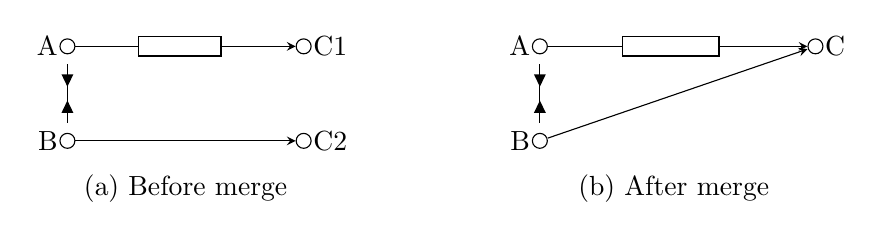
\begin{tikzpicture}
\ionode{(io1)}{(-5,1.2)}{node[left]{A}}
\ionode{(io2)}{(-5,0)}{node[left]{B}}
\ionode{(io3)}{(-2,1.2)}{node[right]{C1}}
\ionode{(io4)}{(-2,0)}{node[right]{C2}}
\syncdrain{(io1)}{(io2)}{}
\fifoe{(io1)}{(io3)}{}
\sync{(io2)}{(io4)}{}
\draw (-3.5, -0.6) node[draw=none] {(a) Before merge};
%\draw (-1.6, -0.6) node[draw=none] {Transformed version of alternator.};

\ionode{(io1)}{(1,1.2)}{node[left]{A}}
\ionode{(io2)}{(1,0)}{node[left]{B}}
\ionode{(io3)}{(4.5,1.2)}{node[right]{C}}
%\ionode{(io4)}{(5,0)}{node[right]{C2}}
\syncdrain{(io1)}{(io2)}{}
\fifoe{(io1)}{(io3)}{}
\sync{(io2)}{(io3)}{}
\draw (2.7, -0.6) node[draw=none] {(b) After merge};
\end{tikzpicture}
\caption{Alternator}
\label{fig:alternator}
\end{figure}

Here the replicate operation has been applied twice for the alternator: node \emph{A} becomes the common source node of \emph{Syncdrain (A,B)} and \emph{FIFO1(A,C1)}, and node \emph{B} becomes the common source node of \emph{Syncdrain(A,B)} and \emph{Sync(B,C2)}. Let the time streams when the
data streams flow into the two source nodes \emph{A} and \emph{B} be denoted by \emph{a} and \emph{b}, and the time streams when the data streams
flow out of the channels \emph{FIFO1(A,C1)} and \emph{Sync(B,C2)} be denoted by \emph{c1} and \emph{c2}, respectively. Theorem \ref{the:alternator}
specifies the property $c2<c1 \wedge c1<tl (c2)$ of the connector in Fig. \ref{fig:alternator}(a). The connector is based on the axioms
Sync, Syncdrain and FIFO1. These three corresponding axioms are used as hypotheses for the proof of this theorem.
\begin{theorem}[subtest]\label{the:alternator}
$\forall A,B,C1,C2.$
\begin{eqnarray*}
  & SyncDrain(A,B)\land FIFO1(A,C1)\land Sync(B,C2)  \rightarrow & \\
  & Tle(C2,C1) \wedge Tle(C1, tl(C2))
\end{eqnarray*}
\end{theorem}
In Coq, the theorem can be proved as follows. Note that the formalizm is slightly different from the previous one. By the \emph{section} environment, Coq is able to encapsulate hypothesises as assumptions of the theorem. So the two definitions are exactly equivalent.

\begin{verbatim}
    Section Alt.
    Hypothesis D1: SyncDrain A B.
    Hypothesis D2: FIFO1 A C1.
    Hypothesis D3: Sync B C2.
    Theorem subtest:
       (Tle C2 C1)  /\  (Tle C1 (tl C2)).
\end{verbatim}

After constructing the connector in Fig. \ref{fig:alternator}(a), we use ``destruct" to obtain the conditions for time and data, respectively.
Since the goal we are going to prove is an intersection of logical predicates, we use ``split" to obtain the single subgoals represented by
logical predicates. Besides, ``intros" contributes to comparing each data in a sequence element by element. Then ``rewrite" and ``apply" are
used similarly for multiple times until the goal is proved finally. %We can see that a new tactic named \emph{split} is used in the proof of
%this property.
Concrete proof steps and feedbacks are specified in Table \ref{tb:proof}.

\begin{table}[ht]
\label{tb:proof}
\newcommand{\tabincell}[2]{\begin{tabular}{@{}#1@{}}#2\end{tabular}}
  \centering
  \scriptsize
  \caption{Steps and feedback}
  \begin{tabular}{|c|c|c|}\hline
\tabincell{c}{Step} & \tabincell{c}{Feedback}\\\hline
\tabincell{c}{Theorem subtest%:\\((Tle C2) C1) $\wedge$ ((Tle C1) (tl C2))
}
   & \tabincell{c}{ 1 subgoal: \emph{Tle C2 C1 $\wedge$ Tle C1 (tl C2)}} \\\hline
\tabincell{c}{destruct \emph{D2} } & \tabincell{c}{ 1 subgoal: \emph{Tle C2 C1 $\wedge$ Tle C1 (tl C2)}
 \\ \emph{H : Tle A C1;
H0 : Tle C1 (tl A) $\wedge$ Deq A C1}} \\\hline
\tabincell{c}{destruct \emph{D3} } & \tabincell{c}{ 1 subgoal: \emph{Tle C2 C1 $\wedge$ Tle C1 (tl C2)}
 \\\emph{H : Tle A C1;
H0 : Tle C1 (tl A) $\wedge$ Deq A C1;}\\
\emph{H1 : Teq B C2;
H2 : Deq B C2}} \\\hline
\tabincell{c}{
destruct \emph{H0}} & \tabincell{c}{ 1 subgoal: \emph{Tle C2 C1 $\wedge$ Tle C1 (tl C2)}
\\\emph{H : Tle A C1;
H0 : Tle C1 (tl A);}\\
\emph{H3 : Deq A C1;
H1 : Teq B C2;
H2 : Deq B C2}} \\\hline
\tabincell{c}{split } & \tabincell{c}{2 subgoals: \emph{Tle C2 C1; Tle C1 (tl C2)}\\ \emph{H : Tle A C1;
H0 : Tle C1 (tl A);}\\
\emph{H3 : Deq A C1;
H1 : Teq B C2;
H2 : Deq B C2}} \\\hline
\tabincell{c}{intros $n$ } & \tabincell{c}{ 2 subgoals: \emph{PrL (Str\_nth n C2) $<$ PrL (Str\_nth n C1); Tle C1 (tl C2)} \\
\emph{H : Tle A C1;
H0 : Tle C1 (tl A);
H3 : Deq A C1;}\\
\emph{H1 : Teq B C2;
H2 : Deq B C2;
n : nat}
} \\\hline
\tabincell{c}{rewrite  $\leftarrow$ \emph{H1} } & \tabincell{c}{ 2 subgoals: \emph{PrL (Str\_nth n B) $<$ PrL (Str\_nth n C1); Tle C1 (tl C2)}\\
\emph{H : Tle A C1;
H0 : Tle C1 (tl A);
H3 : Deq A C1;}\\
\emph{H1 : Teq B C2;
H2 : Deq B C2;
n : nat}} \\\hline
\tabincell{c}{rewrite  $\leftarrow$ \emph{D1} } & \tabincell{c}{ 2 subgoals: \emph{PrL (Str\_nth n A) $<$ PrL (Str\_nth n C1); Tle C1 (tl C2)}\\
\emph{H : Tle A C1;
H0 : Tle C1 (tl A);
H3 : Deq A C1;}\\
\emph{H1 : Teq B C2;
H2 : Deq B C2;
n : nat}} \\\hline
\tabincell{c}{apply \emph{H} } & \tabincell{c}{ 1 subgoal: \emph{Tle C1 (tl C2)} \\ \emph{H : Tle A C1;
H0 : Tle C1 (tl A);
H3 : Deq A C1;}\\
\emph{H1 : Teq B C2;
H2 : Deq B C2}} \\\hline
\tabincell{c}{intros $n$ } & \tabincell{c}{ 1 subgoal: \emph{Tle C1 (tl C2)} \\ \emph{H : Tle A C1;
H0 : Tle C1 (tl A);
H3 : Deq A C1;}\\
\emph{H1 : Teq B C2;
H2 : Deq B C2}} \\\hline
\tabincell{c}{rewrite  $\leftarrow$ \emph{D4} } & \tabincell{c}{ 2 subgoals: \emph{PrL (Str\_nth n C1) $<$ PrL (Str\_nth n (tl B)); Teq B C2}\\
\emph{H : Tle A C1;
H0 : Tle C1 (tl A);
H3 : Deq A C1;}\\
\emph{H1 : Teq B C2;
H2 : Deq B C2;
n : nat}} \\\hline
\tabincell{c}{rewrite  $\leftarrow$ \emph{D5} } & \tabincell{c}{ 3 subgoals: \emph{PrL (Str\_nth n C1) $<$ PrL (Str\_nth n (tl A)); Teq A B; Teq B C2}\\
\emph{H : Tle A C1;
H0 : Tle C1 (tl A);
H3 : Deq A C1;}\\
\emph{H1 : Teq B C2;
H2 : Deq B C2;
n : nat}} \\\hline
\tabincell{c}{apply \emph{H0} } & \tabincell{c}{ 2 subgoals: \emph{Teq A B; Teq B C2} \\ \emph{H : Tle A C1;
H0 : Tle C1 (tl A);
H3 : Deq A C1;}\\
\emph{H1 : Teq B C2;
H2 : Deq B C2;
n : nat}} \\\hline
\tabincell{c}{apply \emph{D1} } & \tabincell{c}{ 1 subgoal: \emph{Teq B C2} \\ \emph{H : Tle A C1;
H0 : Tle C1 (tl A);
H3 : Deq A C1;}\\
\emph{H1 : Teq B C2;
H2 : Deq B C2;
n : nat}} \\\hline
\tabincell{c}{apply \emph{D3}} & \tabincell{c}{ No more subgoals.} \\\hline
\end{tabular}
\end{table}

The proof of Theorem \ref{the:alternator} for the connector in Fig. \ref{fig:alternator}(a) can be used to simplify the proof for the following
property of alternator.

An additional hypothesis is needed for the proof of alternator which merges \emph{C1} and \emph{C2} into a common node \emph{C}. Based on the three
hypotheses for channels and the additional hypothesis, the theorem of alternator is presented as the following proposition which needs to be proved:
\begin{verbatim}
    Hypothesis D4: merge C1 C2 C.
    Theorem test:
    hd(C) = hd(C2) /\ merge C1 (tl C2) (tl C).
    Proof.
      destruct subtest.  (* ... *)
\end{verbatim}
Here we only present the first step which shows how a proven theorem can be applied in another proof and omit the full details because of the page limitation.
And it greatly simplifies the process of proving the property of alternator.
\end{example}

\subsection{Refinement and Equivalence}

A refinement relation between connectors which allows us to systematically develop connectors in a step-wise fashion, may help to bridge
the gap between requirements and the final implementations. The notion of refinement has been widely used in different system descriptions.
For example, in data refinement\cite{RE98}, the `concrete' model is required to have \emph{enough redundancy} to represent all the elements
of the `abstract' one. This is captured by the definition of a surjection from the former into the latter (the \emph{retrieve map}). If
models are specified in terms of pre and post-conditions, the former are weakened and the latter strengthened under refinement \cite{Jon90}.
In process algebra, refinement is usually discussed in terms of several `observation' preorders, and most of them justify
transformations entailing \emph{reduction of nondeterminism} (see, for
example, \cite{Ros98}). For connectors, the refinement relation can be
defined as in \cite{SAA+12}, where a proper refinement order over
connectors has been established based on the implication relation on
predicates.

%Based on our connector models in Coq, the implication relation on predicates establishes a proper refinement order over connectors.
%Generally speaking, a formal model \emph{A} refines another model \emph{B} means that \emph{B} contains more behavior than \emph{A}.
Here we adopt the definition of refinement in \cite{SAA+12}. Two connectors are equivalent if each one of them is a refinement of the other.
In the following, we show two examples of such connector refinement and equivalence relations.

\begin{example}[Refinement]
\label{ex:refine}
Taking the two connectors in Fig. \ref{refine} into consideration, connector \emph{Q} is a refinement of connector \emph{P} (denoted by $\emph{P} \sqsubseteq \emph{Q}$).
\begin{figure}
\vspace{0cm}
\centering
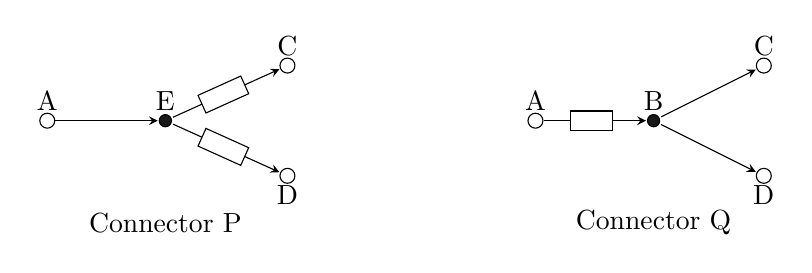
\begin{tikzpicture}
\ionode{(io4)}{(5,1.0)}{node[above]{A}}
\ionode{(io5)}{(7.9,1.7)}{node[above]{C}}
\ionode{(io6)}{(7.9,0.3)}{node[below]{D}}
\mixednode{(m2)}{(6.5,1.0)}{node[above]{B}}
\draw (6.5, -0.3) node[draw=none] {Connector Q};

\ionode{(io1)}{(-1.2,1.0)}{node[above]{A}}
\ionode{(io2)}{(1.85,1.7)}{node[above]{C}}
\ionode{(io3)}{(1.85,0.3)}{node[below]{D}}
\mixednode{(m1)}{(0.3,1.0)}{node[above]{E}}
\draw (0.3, -0.3) node[draw=none] {Connector P};


\sync{(io1)}{(m1)}{}
\fifoe{(m1)}{(io2)}{}
\fifoe{(m1)}{(io3)}{}

\sync{(m2)}{(io5)}{}
\sync{(m2)}{(io6)}{}
\fifoe{(io4)}{(m2)}{}
\end{tikzpicture}
\caption{Example of connector refinement}
\label{refine}
\end{figure}

We have mentioned that newly constructed connectors can be specified as theorems. Given arbitrary input timed
data stream at node \emph{A} and output timed data streams at nodes \emph{C}, \emph{D}, essentially connector
\emph{Q} is a refinement of another connector \emph{P} only if the behavior property of \emph{P} can
be derived from \emph{theorem Q}, i.e., the property of connector \emph{Q}. Intuitively, connector \emph{P} enables the
data written to the source node \emph{A} to be asynchronously taken out via the two sink nodes \emph{C} and \emph{D}, but
it has no constraints on the relationship between the time of the two output events. On the other hand,
connector \emph{Q} refines this behavior by synchronizing the two sink nodes, which means that the two output
events must happen simultaneously. To be more precise, we use \emph{c,d} to denote the time streams of the two outputs
and \emph{a} to denote the time stream of the input. Connector \emph{P} satisfies condition $a<c\wedge a<d$ and
connector \emph{Q} satisfies $a<c\wedge a<d \wedge c=d$.

The refinement relation can be formally defined in Coq as:

%\begin{theorem}[refinement]
%$\forall A,C,D$:
%\begin{eqnarray*}
%\exists B. FIFO1(A,B)\wedge Sync(B,C)\wedge Sync(B,D) & \rightarrow & \\
%\exists E. Sync (A,E) \wedge FIFO1 (E,C) \wedge FIFO1 (E,D)
%\end{eqnarray*}
%\end{theorem}


\begin{verbatim}
    Theorem refinement : forall A C D,
    (exists B, (FIFO1 A B) /\ (Sync B C) /\ (Sync B D)) ->
    (exists E, (Sync A E) /\ (FIFO1 E C) /\ (FIFO1 E D)).
\end{verbatim}


% Specifically, the refinement relation in this example can be formally represented as the following implication relation:
%  \begin{eqnarray*}
%    \forall B_{0}.FIFO1(A,B_{0})\wedge Sync(B_{0},C)\wedge Sync(B_{0},D) & \rightarrow &  \\
%    \exists B.Sync(A,B)\wedge FIFO1(B,C) \wedge FIFO1(B,D)
%  \end{eqnarray*}

To prove this refinement relation, we first introduce a lemma which is frequently used in the proof.
\begin{lemma}[Eq]\label{lemma:eq}
$\forall$A,B: Stream TD.
  Sync (A,B) $\Leftrightarrow$ A$=$B.
\end{lemma}
The lemma means that \emph{Sync(A,B)} and \emph{A$=$B} can be derived
from each other. Although this lemma seems to make the presence of
Sync channels in connectors redundant, it is not the case for most
connectors. For example, if we consider
the alternator in Example 2, it can not accept any input data if we
remove the synchronous channel \emph{BC} and use one node for it.

By using the axioms for the basic channels and the operators of composition, we can obtain the two connectors easily.
In the process of constructing the connectors, the flow-through and replicate operations act once for each connector, respectively.


\begin{figure}[htbp]
\centering
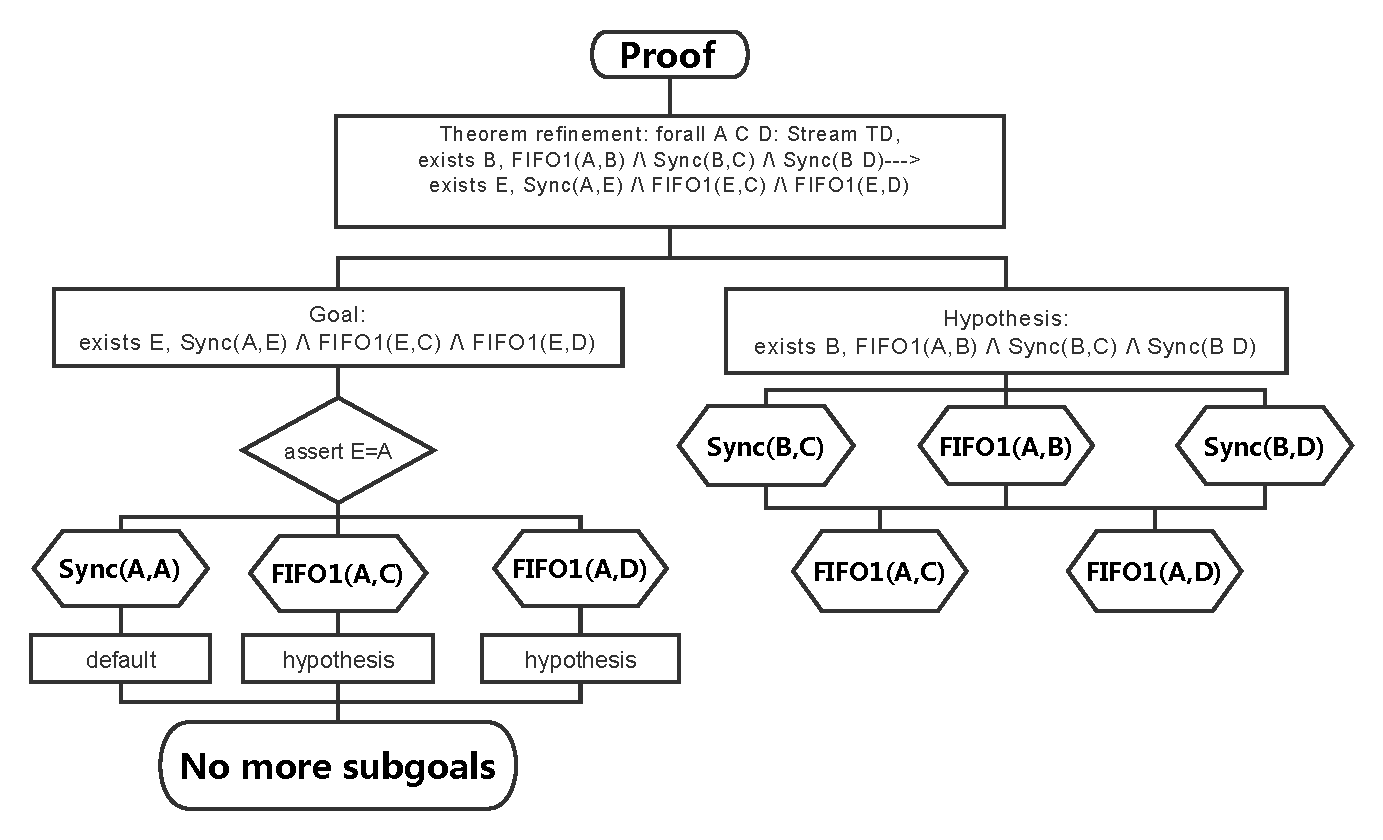
\includegraphics[width=11cm]{Refinement.pdf}
\caption{Proof Steps Flow Chart}
\label{fig:equivalence}
\end{figure}

Fig. \ref{fig:equivalence} shows the flow chart for the proof steps of
connector refinement in this example.


We now show the specific tactics used in the proof of refinement
$\emph{P} \sqsubseteq \emph{Q}$ for connectors \emph{P} and \emph{Q}
in this example.
We need to find a timed data stream which specifies the data-flow through node \emph{E} of connector \emph{P}, i.e., we need to find an appropriate \emph{$E$} that satisfies $Sync(A,E)\wedge FIFO1(E,C) \wedge FIFO1(E,D)$.

First we employ `intros' to acquire a simpler subgoal $\exists E_{0}. Sync(A,E_{0})
\wedge FIFO1(E_{0},C) \wedge FIFO1(E_{0},D)$. Then we assert that \emph{E} $=$ \emph{A}.% which leads to  $Sync(A,A)\wedge FIFO1(A,C) \wedge FIFO1(A,D)$.
After using `split', we split the goal into two subgoals \emph{Sync (A, E)} and \emph{FIFO1 (E, C) $\wedge$ FIFO1 (E, D)}. And by `rewrite' \emph{$H_{0}$ ($H_{0}$: E $=$ A)}, we replace the two subgoals with \emph{Sync (A, A)} and \emph{FIFO1 (E, C) $\wedge$ FIFO1 (E, D)}, respectively.

Through `apply' Lemma \ref{lemma:eq} (\emph{Eq}), we have \emph{A $=$ A} in place of \emph{Sync (A, A)}. Next the tactic \emph{reflexivity} makes the subgoal \emph{A $=$ A} proved directly. Up to now, the initial subgoal \emph{Sync (A, E)} has been achieved.

Using `split' again, the remaining unproven subgoal is split into two subgoals \emph{FIFO1 (E, C)} and \emph {FIFO1 (E, D)}.
After destructing the precondition three times, we succeed in obtaining three hypotheses: \emph{ H: FIFO1 (A, x); H1: Sync (x, C); H2: Sync (x, D)}. Assume x $=$ C and then using tactics \emph{apply Eq} and \emph{assumption}, \emph{assertion x $=$ C} is proved easily. Meanwhile, we get hypothesis \emph{H3: x $=$ C}. Via \emph{Rewrite $\leftarrow$H3}, we bring left in place of the right side of the equation \emph{H3: x = C} into \emph{FIFO1 (E, C)} and have \emph{FIFO1 (E, x)}. Similarly, rewrite \emph{H0} and further we get the result \emph{FIFO1 (A, x)} which is exactly hypothesis \emph{H}. By using `assumption', the second subgoal is proved already.
Using substantially the same tactic steps, \emph{FIFO1 (E, D)} can be proved. Finally, we have no more subgoals. Note that there is a new tactic `reflexivity' used in the proof, which is actually synonymous with `apply refl equal'. We can use it to prove that two statements are equal.

\end{example}

\begin{example}[Equivalence]
%When connector \emph{P} is a refinement of  connector \emph{Q} and \emph{Q} is a refinement of \emph{P}, we say that connector \emph{P} and \emph{Q} is equivalent.
For the connector \emph{P} in Example \ref{ex:refine}, we can add three more basic channels to build a new connector \emph{R} which is equivalent to \emph{Q}. \emph{R} can be interpreted similarly based on basic channels and operators. We will omit the details for its construction here and prove the equivalence between the two connectors \emph{R} and \emph{Q} directly.
%The specific channels and operators used to construct the new connector will not be repeated here. Next we will prove the equivalence of the two connectors.

\begin{figure}
\vspace{0cm}
\centering
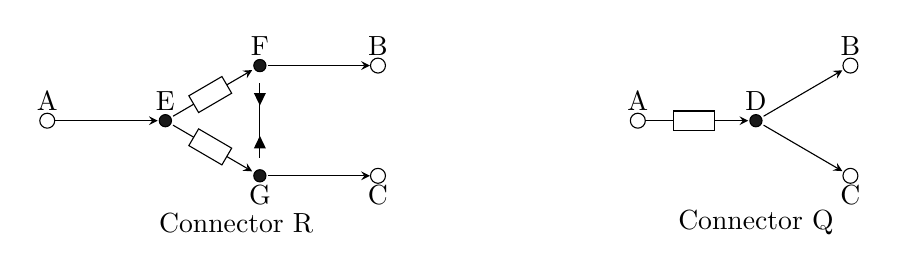
\begin{tikzpicture}
\ionode{(io4)}{(3.5,1.0)}{node[above]{A}}
\ionode{(io5)}{(6.2,1.7)}{node[above]{B}}
\ionode{(io6)}{(6.2,0.3)}{node[below]{C}}
\mixednode{(m2)}{(5,1.0)}{node[above]{D}}
\draw (5, -0.3) node[draw=none] {Connector Q};

\ionode{(io1)}{(-4,1.0)}{node[above]{A}}
\ionode{(io2)}{(0.2,1.7)}{node[above]{B}}
\ionode{(io3)}{(0.2,0.3)}{node[below]{C}}
\mixednode{(m1)}{(-2.5,1.0)}{node[above]{E}}
\mixednode{(m3)}{(-1.3,1.7)}{node[above]{F}}
\mixednode{(m4)}{(-1.3,0.3)}{node[below]{G}}
\draw (-1.6, -0.3) node[draw=none] {Connector R};

\sync{(io1)}{(m1)}{}
\fifoe{(m1)}{(m3)}{}
\fifoe{(m1)}{(m4)}{}
\sync{(m3)}{(io2)}{}
\sync{(m4)}{(io3)}{}
\syncdrain{(m3)}{(m4)}{}


\sync{(m2)}{(io5)}{}
\sync{(m2)}{(io6)}{}
\fifoe{(io4)}{(m2)}{}


\end{tikzpicture}
\caption{Example of connector equivalence}
\label{refine1}

\end{figure}

Equivalence relationship between the two connectors can be formalized as:
\begin{verbatim}
    Theorem equivalence: forall A B C,
      (exists E F G,
        (Sync A E) /\ (FIFO1 E F) /\ (Sync F B) /\
        (FIFO1 E G) /\ (Sync G C) /\ (SyncDrain F G)
      ) <->
      (exists D,
        (FIFO1 A D) /\ (Sync D B) /\ (Sync D C)
      ).
\end{verbatim}
The proof of this theorem has two steps. Firstly, we prove that the new connector \emph{R} is a refinement of connector \emph{Q}.
We hope to find an appropriate \emph{$D$} that satisfies
\[
FIFO1(A,D)\wedge Sync(D,B) \wedge Sync(D,C)
\]
Similar to Example \ref{ex:refine}, we first assert $D=F$, which leads to
\[
FIFO1(A,F) \land Sync(F,B) \wedge Sync(F,C)
\]
From Lemma \ref{lemma:eq}, we have $Sync(A,E)$, or $A=E$. Therefore, \emph{FIFO1(E,F)} can be replaced by \emph{FIFO1(A,F)}. By adopting \emph{FIFO1(E,F)} and \emph{FIFO1(E,G)}, we can prove that the data sequences at \emph{F} and \emph{G} are equal. Similarly, data sequences at $C$, $G$ and $F$ are also equal, wrt. $Sync(G,C)$.

Further according to \emph{Sync(G,C)} and \emph{Syncdrain(F,G)}, the time sequences at \emph{F} and \emph{C} are proved equal. With the combination of relations on time and data between \emph{F} and \emph{C}, we can draw the conclusion \emph{Sync(F,C)}.


Up to now, we present a proof for \emph{Sync(F,C)} and \emph{FIFO1(A,F)} by the derivation. Besides, \emph{Sync(F,B)} is already declared in the assumptions. Consequently, the refinement relation has been proved.

Secondly, we prove that connector \emph{Q} is a refinement of connector \emph{R}.
We hope to find appropriate timed data streams at \emph{E,F,G}  which satisfy
\begin{eqnarray*}
\emph{Sync(A,E)}&\wedge& \emph{Sync(G,C)} \wedge \emph{FIFO1(E,G)}\wedge \emph{Sync(F,B)}\\
 &\wedge& \emph{FIFO1(E,F)}\wedge \emph{Syncdrain(F,G)}.
\end{eqnarray*}
We can directly assume $E=A$, $F=D$ and $G=D$. Now we only need to prove
\emph{Sync(A,A)} $\wedge$  \emph{Sync(D,C)}  $\wedge$  \emph{FIFO1(A,D)} $\wedge$  \emph{Sync(D,B)} $\wedge$ \emph{FIFO1(A,D)} $\wedge$ \emph{Syncdrain(D,D)}, which can be easily derived from the assumptions.
\end{example}

\section{Refinement Checking} \label{sec:refinement}
Modelling and reasoning of Reo connectors in Coq can only provide a proof of that one connector is indeed a refinement of the other connector when coming to refinement checking, although it allows us to reason about a relatively wide range of properties. Moreover, the refinement relation is a fairly important part of properties, which is used in many applications. Therefore, in order to fulfil the proof of the refinement relation, Z3 solver is needed as an assistant tool, particularly applied to refinement checking.
\subsection{Basic Channels}
Before using Z3 to fulfil the proof of refinement relation, we need to implement the construction of connectors and also define the refinement checking function in a way that fits in with Z3 solver. Typically, connector construction starts with the definition of basic channels and composition operators. The formalization of basic framework is important and primary, so that we can further formalize our reasoning within this model.

Coinciding with the definition of channels in Coq, we dealt with both time and data relation constraints in the basic definition. An auxiliary function \emph{Conjunction} is used to take the conjunction of every constraint in the constraint lists parameterized by \emph{constraints}.

By means of function \emph{Conjunction}, basic channels are defined concisely and neatly. But the biggest difference is that what we feed Z3 solver need to be constraints such that Z3 solver can make decisions and yield results about refinement relations between connectors. For example, the specific behavior constraints for \emph{Sync} channel are classified into two types: data constraints and time constraints. The description and the definition of \emph{Sync} in Coq have already clearly expressed the behavior pattern it needs to follow: each item in data and time streams of output specified as ``node[1]'' is equivalent to the data and time streams of input specified as ``node[0]'', which are exactly data and time constraints. As they are both requirements we need to satisfy no matter data or time is related, each constraint in the list will all be merged finally.
\lstset{language=Python}
\begin{lstlisting}[frame=single]
def Sync(nodes, bound):
   assert len(nodes) == 2
   constraints = []
   for i in range(bound):
     constraints += [ nodes[0]['data'][i] == nodes[1]['data'][i] ]
     constraints += [ nodes[0]['time'][i] == nodes[1]['time'][i] ]
   return Merge(constraints)
\end{lstlisting}

\emph{Syncdrain} and \emph{FIFO1} channel are defined in a similar way. On the basis of the behavior of \emph{Syncdrain} channel, there are only time related constraints to be needed, i.e., equivalence of each item in two time streams of the two inputs. Regarding \emph{FIFO1} channels, constraints related data is the same as \emph{Sync} channels. But there are more time related constraints. As the buffer capacity is one, the relation of each item in the input time stream and output time stream need to be carefully dealt with, especially that the next input should be later than the output at present. At last, their corresponding constraint lists consist of constraint statements similar to the statements above.
\begin{lstlisting}[frame=single]
def SyncDrain(nodes, bound):
   assert len(nodes) == 2
   constraints = []
   for i in range(bound):
       constraints +=
            [nodes[0]['time'][i] == nodes[1]['time'][i]]
   return Merge(constraints)
\end{lstlisting}
\begin{lstlisting}[frame=single]
def Fifo1(nodes, bound):
   assert len(nodes) == 2
   constraints = []
   for i in range(bound):
      constraints +=
                  [ nodes[0]['data'][i] == nodes[1]['data'][i] ]
      constraints +=
                  [ nodes[0]['time'][i] <  nodes[1]['time'][i] ]
      if i:
          constraints +=
                  [ nodes[0]['time'][i] > nodes[1]['time'][i-1] ]

   return Merge(constraints)
\end{lstlisting}

In accordance with the behavior of \emph{Lossy} channel, each item of the input stream may or may not be lost. If so, then the output gets nothing. If not, it behaves exactly like \emph{Sync} channel, so in this case the data and time related constraints are identical with those in the definition of \emph{Sync} channel. The biggest difference is that \emph{Lossy} channel should be defined in a recursive way according to its own distinctive behavior. Note that the constraints are added in a recursive way which is in great coincidence with the original definition.
\begin{lstlisting}[frame=single]
def Lossy(nodes, bound, idx = 0, num = 0):
   assert len(nodes) == 2
   if bound == num:
     return True
   if bound == idx:
     return True
   constraints_0 = []
   constraints_1 = []
   constraints_0 +=
           [ nodes[0]['data'][idx] != nodes[1]['data'][num]]
   constraints_0 +=
           [ nodes[0]['time'][idx] != nodes[1]['time'][num]]
   constraints_1 +=
           [ nodes[0]['data'][idx] == nodes[1]['data'][num]]
   constraints_1 +=
           [ nodes[0]['time'][idx] == nodes[1]['time'][num]]
   return Or(And(Merge(constraints_0),
             Channel.Lossy(nodes, bound, idx + 1, num)),
             And(Merge(constraints_1),
             Channel.Lossy(nodes, bound, idx + 1, num + 1))
             )
\end{lstlisting}
\subsection{Composition Operators}
While the basic channels are already well defined as the basis of the whole construction framework, the composition operators also need to be specified for the large-scale connector construction just like cement for bricks.

Among the three types of composition operators, the most important and difficult one is \emph{Merge}, which is specially dealt with as a channel \emph{Merger} in our model. Although the composition operator \emph{Merge} is treated as a channel \emph{Merger}, it also play the same part in the construction of a connector.  Plus the rest of composition operators: \emph{replicate} and \emph{flow-through}, they are enough for the whole construction for any connector, which can serve as same as the original composition operations. For each item of output stream, there is a nondeterministic choice between the two input nodes. Hence, the \emph{Merger} channel also need to be defined in a recursive way like \emph{Lossy} channel. Note that the constraints also conform well to the original definition of \emph{Merge}. Concluded from the two recursive definitions, an additional advantage of defining \emph{Lossy} and \emph{Merger} channel in this way is that it can preserve the behavioral pattern to a great extent without many assumptions such as priorities of reading or taking data.
\begin{lstlisting}[frame=single]
def Merger(nodes, bound, idx_1 = 0, idx_2 = 0):
   assert len(nodes) == 3
   if bound == idx_1 + idx_2:
     return True
   constraints_1 = []
   constraints_2 = []
   constraints_1 +=
    [ nodes[0]['data'][idx_1] == nodes[2]['data'][idx_1 + idx_2]]
   constraints_1 +=
    [ nodes[0]['time'][idx_1] == nodes[2]['time'][idx_1 + idx_2]]
   constraints_1 +=
    [ nodes[0]['time'][idx_1] <  nodes[1]['time'][idx_2]]
   constraints_2 +=
    [ nodes[1]['data'][idx_2] == nodes[2]['data'][idx_1 + idx_2]]
   constraints_2 +=
    [ nodes[1]['time'][idx_2] == nodes[2]['time'][idx_1 + idx_2]]
   constraints_2 +=
    [ nodes[1]['time'][idx_2] <  nodes[0]['time'][idx_1]]
   return Or(And(Merge(constraints_1),
             Channel.Merger(nodes, bound, idx_1 + 1, idx_2)),
             And(Merge(constraints_2),
             Channel.Merger(nodes, bound, idx_1, idx_2 + 1))
             )
\end{lstlisting}
\emph{Replicate} and \emph{flow-through} operators are implicitly achieved when we compose channels to construct connectors using the same node names. A simple example for the implementation of \emph{replicate} is \emph{c1.connect(`Sync', `A', `E'), c1.connect(`Fifo1', `E', `F'), c1.connect(`Fifo1', `E', `G')} where message from node `E' is copied to send to nodes `F' and `G' simultaneously. As for \emph{flow-through} operator, a simple example is \emph{c2.connect(`Fifo1', `A', `D'), c2.connect(`Sync', `D', `B')} where the timed data flows from node `A' to node `B' through the mixed node `D'. In these two simple examples, \emph{c1} and \emph{c2} both belong to connector class which will be elaborated in detail in next module.
\subsection{Reasoning about refinement relation}
With basic channels and composition operators well formulated above, we are left with the task of first constructing Reo connectors. In this model, connector is defined as a new class, which provides a method of constructing complex connectors out of channels and operators.
The statements inside a class definition are function definitions. We have seen the function `connect' used in the two simple examples of \emph{replicate} and \emph{flow-through}.
\begin{lstlisting}[frame=single]
class Connector:
    def __init__(self):
        self.channels = []

    def connect(self, channel, *nodes):
        self.channels += [(channel, nodes)]
        return self
\end{lstlisting}
Another function \textbf{\emph{isRefinementOf}} is the most crucial one in refinement checking. The result of the function \textbf{\emph{isRefinementOf}} is Boolean, i.e., a connector either is or not a refinement of another connector. According to the definition of refinement relation in section \ref{sec:verification}, we have a formula to represent it properly: $Q \rightarrow P$ if and only if the behavior property of \emph{P} can be derived from the property of connector \emph{Q}, i.e., $\emph{P} \sqsubseteq \emph{Q}$. The background theory of the definition of function  \textbf{\emph{isRefinementOf}} is based on first order logic. Initially, if \emph{Q} is indeed a refinement of \emph{P}, i.e., $Q \rightarrow P$, it can be rephrased as $\neg Q \vee P$. Then, negate it giving $Q \wedge \neg P$. If Z3 solver presents a model satisfying this formula after negation, then the refinement relation is falsified by a counterexample. On the contrary, if there didn't exist a counter example, we may say that the refinement relation, $P\subseteq Q$, holds within the given bound. The formal definition of this function \textbf{\emph{isRefinementOf}} is given as an algorithm here.
\begin{algorithm}[t]
    \caption{Function: P.isRefinementOf (Q, bound)}
    \begin{algorithmic}[1]
        \REQUIRE Both P and Q are connector.
        \ENSURE A boolean: \emph{True} or \emph{False with a counterexample}
        \FOR{channel \emph{t} $\leftarrow$ \emph{P}}
        	\FOR{node \emph{n} $\leftarrow$ \emph{t}}
				\IF{\emph{n} is a new node}
					\STATE i.generate variables like 					
						\newline \{`time':[n\_t\_0, n\_t\_1,...,n\_t\_(bound-1)],				
						\newline `date':[n\_d\_0, n\_d\_1,...,n\_d\_(bound-1)]\}
						\newline
						\newline ii.add time constraints like
						\newline ``n\_t\_0 $\geq$ 0  and  n\_t\_i $<$ n\_t\_i+1''
						\newline into solver
				\ENDIF
			\ENDFOR
		\STATE Add the constraints between different nodes of the same channel into solver according to the property of channels.
        \ENDFOR
        \STATE foralls = []      \% to store new variable
        \STATE absGlobalConstr = None \% to store all constraints under Q
        \STATE absTimeConstr = None \% to store all timed constraints under Q
        \FOR{channel \emph{t} $\leftarrow$ \emph{Q}}
        	\FOR{node \emph{n} $\leftarrow$ \emph{t}}
				\IF{\emph{n} is a new node}
					\STATE i.generate variables like 					
						\newline \{`time':[n\_t\_0, n\_t\_1,...,n\_t\_(bound-1)],				
						\newline `date':[n\_d\_0, n\_d\_1,...,n\_d\_(bound-1)]\}
						\newline
						\newline ii.add \emph{n} into forall
						\newline
						\newline iii.add time constraints like
						\newline ``n\_t\_0 $\geq$ 0  and  n\_t\_i $<$ n\_t\_i+1''
						\newline into absTimeConstr
				\ENDIF
			\STATE add the constraints between different nodes of the same channel into absGlobalConstr according to the property of channels.
			\ENDFOR
		\IF{absTimeConstr is not empty}
			\STATE $absGlobalConstr = \neg (absTimeConstr \cap absGlobalConstr)  $
		\ELSE
			\STATE $absGlobalConstr = \neg absGlobalConstr$
		\ENDIF
		\IF{forall is not empty}
			\STATE apply \emph{ForAll} to absGlobalConstr
			\newline add those constraints into solver
	    \ELSE
	    	\STATE add absGlobalConstr into solver
		\ENDIF	
        \ENDFOR
    \STATE Check.
    \end{algorithmic}
\end{algorithm}

\begin{example}
To get some intuition for this, consider a simple case where \emph{sync = Connector(), sync.connect(`Sync', `A', `B'); fifo1 = Connector(),
fifo1.connect(`Fifo1', `A', `B')}. Two simple connectors which is actually \emph{Sync(A,B)} and \emph{Fifo1(A,B)} have been constructed. Note that a \emph{FIFO1} channel is not a refinement of a \emph{Sync} channel. After invoking the function \textbf{\emph{isRefinementOf}}, we can obtain the result of the refinement relation \emph{fifo1.isRefinementOf(sync)}. The result and the counterexample Z3 solver yields are presented as follows.
\begin{verbatim}
False
A_d_0 = 0, A_d_1 = 0, A_d_2 = 0, A_d_3 = 0, A_d_4 = 0,
A_d_5 = 0, A_d_6 = 0, A_d_7 = 0, A_d_8 = 0, A_d_9 = 0,
A_t_0 = 0, A_t_1 = 2, A_t_2 = 4, A_t_3 = 6, A_t_4 = 8, 
A_t_5 = 10,A_t_6 = 12,A_t_7 = 14,A_t_8 = 16,A_t_9 = 18,
B_d_0 = 0, B_d_1 = 0, B_d_2 = 0, B_d_3 = 0, B_d_4 = 0,
B_d_5 = 0, B_d_6 = 0, B_d_7 = 0, B_d_8 = 0, B_d_9 = 0,
B_t_0 = 1, B_t_1 = 3, B_t_2 = 5, B_t_3 = 7, B_t_4 = 9,
B_t_5 = 11,B_t_6 = 13,B_t_7 = 15,B_t_8 = 17,B_t_9 = 19.
\end{verbatim}
Note that the counterexample is easy to understand. There exists a timed data stream whose time satisfies the constraints of \emph{FIFO1} channel, but don't satisfy the time constraints of \emph{Sync} channel.
\end{example}
\begin{example}
Another simple example is also to seek the refinement relation between two basic channels. The construction is similar to the above example: \emph{sync = Connector(), sync.connect(`Sync', `A', `B'); lossy = Connector(), lossy.connect(`Lossy', `A', `B')}. We know that \emph{Sync} channel is a refinement of \emph{Lossy} channel. When \emph{Lossy} channel behaves well enough to lose any data items, then it behaves exactly like \emph{Sync} channel. On the contrary, \emph{Lossy} channel is not a refinement of \emph{Sync} channel which is consistent with the result \emph{False} given by the Z3 solver. The counterexample is also very intelligible. Note that the first four timed data items were lost with the last timed data item being transferred successfully, which is consistent with the constraints of \emph{Lossy} channel and obviously not in concordance with the constraints of \emph{Sync} channel.
\begin{verbatim}
False
A_d_0 = 2, A_d_1 = 0, A_d_2 = 2, A_d_3 = 3, A_d_4 = 1,
A_t_0 = 0, A_t_1 = 1, A_t_2 = 2, A_t_3 = 3, A_t_4 = 4,
B_d_0 = 1, 
B_t_0 = 4.
\end{verbatim}
\end{example}

Before demonstrating complementary refinement checking between large-scale connectors, we will present some results of bounded refinement and equivalence relation checking in the next two examples.
\begin{example}
\label{ex:equivalence1}
In this example, we consider about the two connectors in Fig.\ref{refine} again. In  Example \ref{ex:refine}, we have seen the refinement relation checking between the two connectors in Coq. However, tactics and strategies can be too professional to comprehend or to tackle with. Although Z3 can only provide a bounded refinement relation checking for these two connectors, it will be much easier to check the refinement relation as we don't need to master concrete theorem proving tactics. All we need to do is to constructing the two connectors in the way accepted by Z3 solver and use the function \emph{isRefinementOf}.
\begin{lstlisting}[frame=single]
c1 = Connector()
c1.connect('Sync', 'A', 'M')
c1.connect('Fifo1', 'M', 'B')
c1.connect('Fifo1', 'M', 'C')

c2 = Connector()
c2.connect('Fifo1', 'A', 'N')
c2.connect('Sync', 'N', 'B')
c2.connect('Sync', 'N', 'C')
\end{lstlisting}
Notice that the \emph{replicate} operator is applied twice in the construction process. Assume the bound is ten and then carry out the function \emph{c2.isRefinementOf(c1, 10)}. Finally, we can get the result \emph{True} which means that \emph{Connector Q} in Fig.\ref{refine} is indeed a refinement of \emph{Connector P}. We can further extend the bound and the time complexity increases linearly as no recursively defined channels are involved.
\end{example}
\begin{example}
This example checks the equivalence relation between connectors in Fig.\ref{refine1}. Construct the two connectors first similar to the example \ref{ex:equivalence1} and invoke the function \emph{isRefinementOf} in two directions. Then we can get the equivalence result.
When giving the bound ten, the results of two directions are both \emph{True}. Hence, we can conclude that the two connectors are in equivalence relation.
\end{example}

\begin{example}
In this example, we will take the well-known Reo connector \emph{Exclusive Router} into consideration. This connector and its variant are shown as follows. The \emph{variant router} is defined like \emph{router} with one major difference: one of the two \emph{Lossy} channels is replaced with a \emph{Sync} channel. Therefore, the behavior of the variant router is actually not exclusive and all data items will be transported to node \emph{E} rather than transmitted to node \emph{E} and \emph{F} exclusively in the original router. Notice that the variant router is a refinement of the original router and conversely not. Construct these two connectors first and set the bound to ten. Invoke the function \emph{isRefinementOf} in two directions, i.e., \emph{c2.isRefinementOf(c1, 10), c1.isRefinementOf(c2, 10)} where \emph{c2} is the variant router. We can find the results Z3 solver yields is \emph{True} and \emph{False} respectively, which is consistent with our intuition.
\begin{figure}
\centering
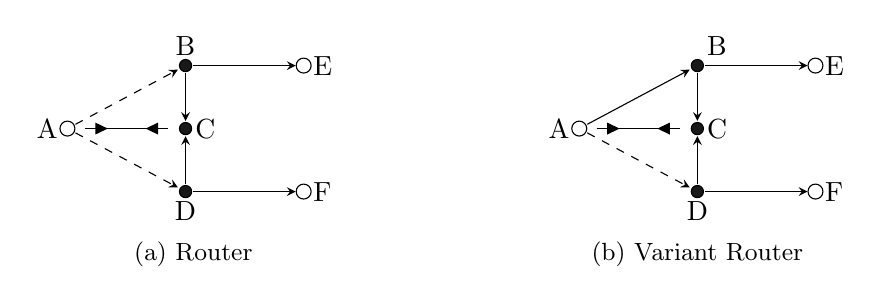
\begin{tikzpicture}
    % part 1. router
    \node (note1) at (6.1, -1.6) {\small (a) Router};
    \node (note2) at (12.5, -1.6) {\small (b) Variant Router};
    \ionode{(in)}{(4.5, 0)}{node[left] {A}}
    \ionode{(outup)}{(7.5, 0.8)}{node[right] {E}}
    \ionode{(outdown)}{(7.5, -0.8)}{node[right] {F}}
    \mixednode{(mid)}{(6, 0)}{node[right] {C}}
    \mixednode{(wayup)}{(6, 0.8)}{node[above] {B}}
    \mixednode{(waydown)}{(6, -0.8)}{node[below] {D}}
    \lossysync{(in)}{(wayup)}{}
    \lossysync{(in)}{(waydown)}{}
    \syncdrain{(in)}{(mid)}{}
    \sync{(wayup)}{(mid)}{}
    \sync{(waydown)}{(mid)}{}
    \sync{(wayup)}{(outup)}{}
    \sync{(waydown)}{(outdown)}{}
    \ionode{(pin)}{(11, 0)}{node[left] {A}}
    \ionode{(poutup)}{(14, 0.8)}{node[right] {E}}
    \ionode{(poutdown)}{(14, -0.8)}{node[right] {F}}
    \mixednode{(pmid)}{(12.5, 0)}{node[right] {C}}
    \mixednode{(pwayup)}{(12.5, 0.8)}{node[above right] {B}}
    %\mixednode{(pmap2)}{(6.5, 1.8)}{node [right] {B'}}
    \mixednode{(pwaydown)}{(12.5, -0.8)}{node[below] {D}}
%    \syncdrain{(pmap2)}{(pwayup)}{}
    \sync{(pin)}{(pwayup)}{}
    \lossysync{(pin)}{(pwaydown)}{}
    \syncdrain{(pin)}{(pmid)}{}
    \sync{(pwayup)}{(pmid)}{}
    \sync{(pwaydown)}{(pmid)}{}
    \sync{(pwayup)}{(poutup)}{}
    \sync{(pwaydown)}{(poutdown)}{}
\end{tikzpicture}
\caption{Example of connector complementary refinement }
\end{figure}


\end{example}
The following large-scale example is aimed at complementary refinement checking.
\subsection{Z3 vs Coq}
Having seen the examples proved by Coq or Z3 solver, we can summarize their features and make a comparison between them.
In the preceding proof about refinement relation or other properties in Coq, the main feature is that users need to master the tactics and strategies well to give a proof of the properties. But there is no need to worry the time consumed in the proof. It will be efficient no matter how large the connectors are as long as users have choose proper tactics. Besides, the connectors whose properties have been proved can be regarded as a theorem when proving properties of much larger ones. Recall that the reason of introducing Z3 solver is that complementary refinement checking, i.e., one connector is not  a refinement of the other one, can't be provided by Coq, let alone provide counterexamples or witnesses.

As we have seen, Z3 solver has shone light on complementary refinement checking. Besides, Z3 solver is much easier to make use of after the definition of the function \emph{isRefinementOf} and the construction framework of Reo connectors compared with using specific tactics and strategies. Moreover, counterexamples and witnesses can be provided as the additional diagnostic feedback while checking the refinement relation between two connectors.
Soundness and completeness of proofs in Z3 solver needs a careful thought. In fact, the biggest drawback of Z3 solver is the failure of ensuring completeness. In simple terms, we didn't provide refinement checking for ideally infinite timed data streams. Nevertheless, it has no influence on the complementary refinement checking, i.e., to prove that one Reo connector is not a refinement of the other connector. As long as we present a counterexample of finite timed data streams, the complementary refinement checking is already done. When it comes to the refinement relation, a finite data stream is not enough to ensure the refinement relation between two Reo connectors for certain. As a result, the equivalence relation is also not ensured completely.

As for time complexity, the efficiency of Z3 solver is well-known. However, proof can be time-consuming when the bound increases gradually, especially for the connectors consisting of one of the two recursively defined channels. When checking complementary refinement relation, the experiments show that a bound limit from 5 to 10 can guarantee a proper counterexample to be given in a reasonable time.
\section{Conclusion and Future Work}\label{sec:conclusion}
In this paper, we present a new approach to model and reason about connectors in the Coq system. The model naturally
preserves the original structure of connectors. This also makes the connector description reasonably readable. We
implement the proof of properties for connectors using identified techniques and tactics provided by Coq. Properties are
defined in terms of predicates which provide an appropriate description of the relation among different
timed data streams on the nodes of a connector. All the analysis and verification work are based on the logical framework
where basic channels are viewed as axioms and composition operations are viewed as operators. As we can address
the relation among different timed data streams, we can easily reason about temporal properties as well as equivalence
and refinement relations for connectors.

As some of the benefits of this approach are inherited from Coq, our approach has also got some of its drawbacks as well.
The main limitation is that the analysis needs much more tactics and techniques when the constructor becomes large.
In the future work, we plan to enhance our framework by two different approaches. Firstly, we may try to encapsulate
frequently-used proof patterns as new tactics, which may reduce lots of repetitive work. After that, automation methods
may also help us to avoid tons of hand-written proof. For example, Coq provides several auto tactics to solve proof
goals. With proper configuration, perhaps such tactics will work well in our framework. More attention is needed to precisely
evaluate how expressive this way is for modeling temporal properties.

\subsection*{Acknowledgement}
\noindent The work was partially supported by the National Natural Science Foundation of China under grant no. 61532019, 61202069 and 61272160.

\bibliographystyle{elsarticle-num}
\bibliography{the}
%\newpage





\end{document}
